\chapter{Badania}
\section{Opis grup pacjentów}
Poniżej szczegółowo zaprezentowano charakterystykę trzech zróżnicowanych grup badawczych. Każda z tych grup została starannie wyselekcjonowana, aby dostarczyć pełniejszego obrazu wpływu aktywności fizycznej na parametry fizjologiczne.
\subsection{Osoby nieaktywne fizycznie}
Grupa osób nieaktywnych fizycznie w ramach badania obejmowała jednostki charakteryzujące się niskim stopniem aktywności fizycznej w ich życiu codziennym. Charakterystyka tej grupy obejmowała:
\begin{itemize}
    \item \textbf{Styl Życia: } Niska aktywność fizyczna w codziennych czynnościach, praca biurowa lub inna forma niewielkiego wysiłku fizycznego oraz brak regularnych sesji treningowych lub aktywności rekreacyjncyh.
    \item \textbf{Stan Zdrowia: } Możliwe występowanie problemów zdrowotnych związanych z brakiem aktywności fizycznej, takich jak nadwaga, obniżona kondycja czy problemy z układem krążenia, Potencjalne ryzyko występowania chorób związanych z brakiem ruchu, takich jak schorzenia sercowo-naczyniowe.
\end{itemize}
\subsection{Kolarze}
Grupa kolarzy składała się z uczestników charakteryzujących się wysokim stopniem aktywności fizycznej, związanym głównie z intensywnym treningiem na rowerze stacjonarnym lub tradycyjnym. Oto specyfika tej grupy:
\begin{itemize}
    \item \textbf{Intensywny Wysiłek Fizyczny: } Regularne i intensywne treningi na rowerze stacjonarnym oraz Długotrwałe sesje treningowe skoncentrowane na poprawie wydolności fizycznej.
    \item \textbf{Styl Życia: } Możliwe zaangażowanie w zawody kolarskie, co może wpływać na intensywność treningów oraz Aktywność fizyczna jako kluczowy element codziennego życia.
\end{itemize}
\subsection{Himalaiści}
Grupa himalaistów składała się z doświadczonych alpinistów, którzy w przeciągu ostatnich 4 miesięcy przynjamniej raz znajdowali się na wysokości powyżej 4000 m n.p.m., charakterystycznych dla wysokich gór. Poniżej przedstawiono charakterystykę tej grupy, ze szczególnym uwzględnieniem ekstremalnych warunków atmosferycznych:
\begin{itemize}
    \item \textbf{Ekstremalne Warunki Treningowe: } Ćwiczenia w warunkach wysokogórskich, gdzie zmniejszone ciśnienie atmosferyczne i niedobór tlenu stwarzają wyjątkowe wyzwania fizjologiczne oraz Trenowanie w warunkach niskich temperatur i zmiennej pogody.
    \item \textbf{Styl Życia: } Częste ekspedycje w wysokie góry, wymagające wytrzymałości fizycznej i psychicznej, jak również Długotrwałe przebywanie w warunkach ekstremalnych, z długimi okresami narażenia na wysokogórskie warunki atmosferyczne.
\end{itemize}
\section{Procedury badawcze}
Procedury badawcze dla trzech wyżej wymienionych grup pacjentów obejmowały szczegółowe pomary parametrów fizjologicznych w warunkach ekstremalnych, charakterystycznych dla środowiska wysokogórskiego. Kroki procedury badawczej zostały przedstawione na grafie poniżej, a następnie opisane szczegółowo.
\begin{figure}[!htb]
    \centering
    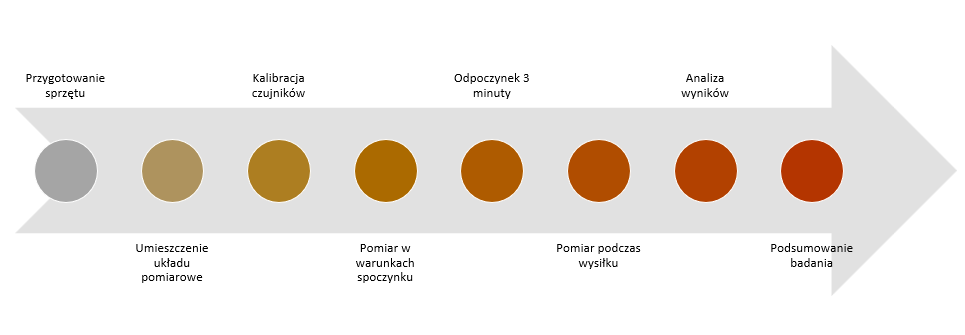
\includegraphics[width=.9\linewidth]{timeline2.png}
    \caption{Oś czasu procedur badawczych}
\end{figure}

Badania rozpoczęto od precyzyjnego przygotowania sprzętu badawczego, obejmującego układ pomiarowy, rower stacjonarny oraz tablet z przygotowaną aplikacją do badania czasu reakcji. Układ pomiarowy został zamocowany na rękawiczce, zapewniając im komfort i swobodę ruchów. Każda badana osoba wykonywała ćwiczenia na jednakowych parametrach rowerka.

Następnie przeprowadzono procedurę kalibracji czujników, aby upewnić się, że dokładnie odzwierciedlają one warunki fizjologiczne osób badanych. Pomiarów parametrów fizjologicznych dokonano zarówno w warunkach spoczynku, jak i podczas treningu (30, 60, 120, 180, 240, 320 sekund) na rowerze stacjonarnym marki Bodymaker. W trakcie badania dynamicznego wszyscy badanii zostali wyposażeni w słomki do oddychania, symulując warunki wysokogórskie. Trening był prowadzony do momentu, kiedy osoba badana odczuwała dyskomfort lub brak sił do dalszego przeprowadzenia treningu, co stanowiło kryterium zakończenia. Ta elastyczność w podejściu do treningu pozwalała dostosować badanie do indywidualnych możliwości i komfortu każdego uczestnika.

Zgromadzone dane poddano analizie w celu porównania różnic w parametrach fizjologicznych w różnych fazach treningu oraz identyfikacji ewentualnych zmian wynikających z warunków atmosferycznych. Podsumowanie wyników badania zawierało wskazanie ewentualnych tendencji, różnic i cennych obserwacji, dostarczając kompleksowej analizy wpływu ekstremalnych warunków górskich na parametry krwi tej grupy.

\begin{figure}[!htb]
    \centering
    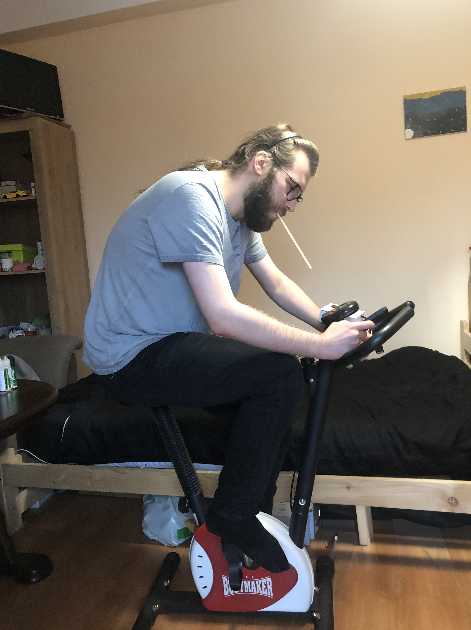
\includegraphics[width=.5\linewidth]{albert.png}
    \caption{Moment badania osoby na rowerku stacjonarnym}
\end{figure}
\newpage
\section{Wyniki}
Poniżej prezentowane są wyniki pomiarów saturacji krwi i fali tętna oraz czasu reakcji, odpowiednio oznaczone SpO2, HR, $\Delta$tRekacji w trzech zróżnicowanych grupach badawczych: osobach nieaktywnych fizycznie, kolarzach oraz himalaistach. Celem analizy było zrozumienie wpływu różnego stopnia aktywności fizycznej na szybkość reakcji organizmu na bodźce, a także ocena adaptacji układu krążenia w kontekście obniżonego poziomu tlenu we krwi.

Wyniki pomiarów zostały zestawione i przedstawione w formie tabelarycznej, umożliwiając szczegółową analizę oraz porównanie między poszczególnymi grupami. Przedstawienie danych w tej formie pozwala na lepsze zrozumienie różnic w reakcjach fizjologicznych w zależności od stopnia aktywności fizycznej, co stanowi istotny wkład w badania nad wpływem aktywności fizycznej na parametry zdrowotne organizmu.
\subsection{Wyniki osób niekatywnych fizycznie}

\begin{table}[ht]
    \centering
    \caption{Tabela wyników osób nieaktywnych fizycznie}
    \begin{tabular}{|c|c|c|c|c|c|c|}
    \hline
                          & Nr. pacjenta        & 1 & 2 & 3 & 4 & 5 \\ \hline
    \multirow{3}{*}{Spoczynek}  & SpO2 $[$\%$]$ & 99   & 99  & 99  & 99  & 99  \\ \cline{2-7} 
                          & HR $[$bpm$]$     & 103  & 71  & 56  & 88  &  83 \\ \cline{2-7} 
                          & $\Delta$tReakcji $[$s$]$  & 1,09  & 1  & 1,74  & 0,89  & 0,94  \\ \hline
    \multirow{3}{*}{30 s}  & SpO2 $[$\%$]$ & 99  & 98  &  98 & 98  &  98 \\ \cline{2-7} 
                          & HR $[$bpm$]$     & 110  &  82 & 78  & 92  & 104  \\ \cline{2-7} 
                          & $\Delta$tReakcji $[$s$]$   & 1,25  & 1,15  & 2,2  & 1,09  & 1,15  \\ \hline
    \multirow{3}{*}{60 s}  & SpO2 $[$\%$]$ & 98  & 96  & 97  & 96  & 97  \\ \cline{2-7} 
                          & HR $[$bpm$]$     & 127  & 94  & 96  & 101  & 130  \\ \cline{2-7} 
                          & $\Delta$tReakcji $[$s$]$   & 1,3  & 1,22  & 1,93  & 1,25  & 1,17  \\ \hline
    \multirow{3}{*}{120 s}  & SpO2 $[$\%$]$ & -  & -  & 94  & 93  & 87  \\ \cline{2-7} 
                          & HR $[$bpm$]$     & -  & -  & 106  & 121  & 140  \\ \cline{2-7} 
                          & $\Delta$tReakcji $[$s$]$   & -  & -  & 2,4  & 2,14  & 1,53  \\ \hline
    \multirow{3}{*}{180 s} & SpO2 $[$\%$]$ &  - & -  & -  & -  & -  \\ \cline{2-7} 
                          & HR $[$bpm$]$     & -  & -  & -  & -  & - \\ \cline{2-7} 
                          & $\Delta$tReakcji $[$s$]$   & -  & -  & -  & -  & -  \\ \hline
    \multirow{3}{*}{240 s} & SpO2 $[$\%$]$ & -  &  - &  - & -  & -  \\ \cline{2-7} 
                          & HR $[$bpm$]$     & -  & -  & -  & -  &  - \\ \cline{2-7} 
                          & $\Delta$tReakcji $[$s$]$   & -  & -  & -  & -  & -  \\ \hline
    \multirow{3}{*}{320 s} & SpO2 $[$\%$]$ & -  &  - &  - & -  & -  \\ \cline{2-7} 
                          & HR $[$bpm$]$     & -  & -  & -  & -  &  - \\ \cline{2-7} 
                          & $\Delta$tReakcji $[$s$]$   & -  & -  & -  & -  &   \\ \hline
    \end{tabular}
    \end{table}

    \newpage
\subsection{Wyniki kolarzy}
\begin{table}[ht]
    \centering
    \caption{Tabela wyników kolarzy}
    \begin{tabular}{|c|c|c|c|c|c|c|}
        \hline
                              & Nr. pacjenta        & 1 & 2 & 3 & 4 & 5 \\ \hline
        \multirow{3}{*}{Spoczynek}  & SpO2 $[$\%$]$ & 99   & 99  & 99  & ----  & ----  \\ \cline{2-7} 
                              & HR $[$bpm$]$     & 69  & 73  & 59  & ----  &  ---- \\ \cline{2-7} 
                              & $\Delta$tReakcji $[$s$]$  & 0,90  & 0,83  & 1,35  & ----  & ----  \\ \hline
        \multirow{3}{*}{30 s}  & SpO2 $[$\%$]$ & 99  & 99  &  99 & ----  &  ---- \\ \cline{2-7} 
                              & HR $[$bpm$]$     & 71  &  77 & 65  & ---- & ----  \\ \cline{2-7} 
                              & $\Delta$tReakcji $[$s$]$   & 0,94  & 0,91  & 1,48  & ----  & ----  \\ \hline
        \multirow{3}{*}{60 s}  & SpO2 $[$\%$]$ & 99  & 99  & 99  & ----  & ----  \\ \cline{2-7} 
                              & HR $[$bpm$]$     & 77  & 79  & 69  & ----  & ----  \\ \cline{2-7} 
                              & $\Delta$tReakcji $[$s$]$   & 0,90  & 0,87  & 1,39  & ----  & ----  \\ \hline
        \multirow{3}{*}{120 s}  & SpO2 $[$\%$]$ & 97  & 98  & 99  & ----  & ---- \\ \cline{2-7} 
                              & HR $[$bpm$]$     & 82  & 82  & 97  & ----  & ----  \\ \cline{2-7} 
                              & $\Delta$tReakcji $[$s$]$   & 1,01 & 0,88  & 1,42  & ----  & ----  \\ \hline
        \multirow{3}{*}{180 s} & SpO2 $[$\%$]$ &  93 & 95  & 94  & ----  & ----  \\ \cline{2-7} 
                              & HR $[$bpm$]$     & 85  & 97  & 91  & ----  & ----  \\ \cline{2-7} 
                              & $\Delta$tReakcji $[$s$]$   & 1,17  & 0,94  & 1,48  & ----  & ----  \\ \hline
        \multirow{3}{*}{240 s} & SpO2 $[$\%$]$ & 90  &  91 &  89 & ----  & ----  \\ \cline{2-7} 
                              & HR $[$bpm$]$     & 87  & 101  & 111  & ----  & ---- \\ \cline{2-7} 
                              & $\Delta$tReakcji $[$s$]$   & 1,14  & 1,03  & 1,58  & ----  & ----  \\ \hline
        \multirow{3}{*}{320 s} & SpO2 $[$\%$]$ & 87  &  86 &  84 & ----  & ----  \\ \cline{2-7} 
                              & HR $[$bpm$]$     & 114  & 119  & 117  & ----  &  ---- \\ \cline{2-7} 
                              & $\Delta$tReakcji $[$s$]$   & 1,22  & 1,09  & 1,69  & ----  & ----  \\ \hline
        \end{tabular}
    \end{table}

\newpage
\subsection{Wyniki himalaistów}
\begin{table}[ht]
    \centering
    \caption{Tabela wyników himalaistów}
    \begin{tabular}{|c|c|c|c|c|c|c|}
        \hline
                              & Nr. pacjenta        & 1 & 2 & 3 & 4 & 5 \\ \hline
        \multirow{3}{*}{Spoczynek}  & SpO2 $[$\%$]$ & 99   & 99  & 99  & 99  & 99  \\ \cline{2-7} 
                              & HR $[$bpm$]$     & 75  & 96  & 87  & 71  &  94 \\ \cline{2-7} 
                              & $\Delta$tReakcji $[$s$]$  & 0,76  & 0,8  & 0,79  & 0,82  & 1,05  \\ \hline
        \multirow{3}{*}{30 s}  & SpO2 $[$\%$]$ &  99 & 99  &  99 & 99  &  99 \\ \cline{2-7} 
                              & HR $[$bpm$]$     & 81  &  101 & 97  & 78  & 99  \\ \cline{2-7} 
                              & $\Delta$tReakcji $[$s$]$   & 1,05  & 0,91  & 0,95  & 0,94  & 1,22  \\ \hline
        \multirow{3}{*}{60 s}  & SpO2 $[$\%$]$ & 99  & 99  & 99  & 99  & 99  \\ \cline{2-7} 
                              & HR $[$bpm$]$   & 100  & 110  & 101  & 92  & 111  \\ \cline{2-7} 
                              & $\Delta$tReakcji $[$s$]$   & 1,03  & 0,92  & 0,92  & 0,95  & 1,15  \\ \hline
        \multirow{3}{*}{120 s}  & SpO2 $[$\%$]$ & 99  & 99  & 99  & 98  & 99  \\ \cline{2-7} 
                              & HR $[$bpm$]$     & 106  & 118  & 115  & 96  & 112  \\ \cline{2-7} 
                              & $\Delta$tReakcji $[$s$]$   & 1,09  & 0,92  & 0,95  & 0,91  & 1,17  \\ \hline
        \multirow{3}{*}{180 s} & SpO2 $[$\%$]$ &  96 & 97  & 99  & 96  & 99  \\ \cline{2-7} 
                              & HR $[$bpm$]$     &  104 & 112  & 111  & 98  & 121  \\ \cline{2-7} 
                              & $\Delta$tReakcji $[$s$]$   & 1,15  & 0,96  & 0,95  & 1,13  & 1,15  \\ \hline
        \multirow{3}{*}{240 s} & SpO2 $[$\%$]$ & 96  &  95 &  96 & 94  & 98  \\ \cline{2-7} 
                              & HR $[$bpm$]$     & 120  & 135  & 135  & 96  &  129 \\ \cline{2-7} 
                              & $\Delta$tReakcji $[$s$]$   & 1,14  & 1,0  & 1,03  & 1,0  & 1,25  \\ \hline
        \multirow{3}{*}{320 s} & SpO2 $[$\%$]$ & 93  &  92 &  95 & 91  & 95  \\ \cline{2-7} 
                              & HR $[$bpm$]$     & 143  & 151  & 132  & 126  &  147 \\ \cline{2-7} 
                              & $\Delta$tReakcji $[$s$]$   & 1,2  & 0,89  & 1,09  & 1,09  & 1,52  \\ \hline
        \end{tabular}
    \end{table}